\documentclass[11pt]{article}
\usepackage{amsmath}
\usepackage{graphicx}
\usepackage{hyperref}

\begin{document}

\title{Cost-Sensitive Regression via Genetic Algorithms}
\author{Team Members: CS21BTECH11060, MA22BTECH11015, AI22BTECH11020}
\maketitle

\section{Introduction}
This report summarizes a cost-sensitive regression implementation using Genetic Algorithms for fraud detection. The dataset consists of 11 independent features (columns A to K), a binary dependent label (column L), and a row-dependent false negative cost (column M). The true positive and false positive costs are constant (6), while the true negative cost is 0.

\section{Methodology}
\subsection{Data Preprocessing}
The data is read from \texttt{costsensitiveregression.csv}. Columns are reordered so that the label becomes the first column and the false negative cost (``FNC'') is separated from the feature set. The dataset is split into training (80\%) and testing (20\%) sets.

\subsection{Cost Functions}
Two cost functions are implemented:
\begin{itemize}
    \item \textbf{Bahnsen Approach:} 
    \[
    L(y, \hat{y}) = y \left(\hat{y} \cdot TP + (1-\hat{y}) \cdot FN\right) + (1-y) \left(\hat{y} \cdot FP + (1-\hat{y}) \cdot TN\right)
    \]
    where \(TP = FP = 6\), \(TN = 0\), and \(FN\) is row-dependent.
    \item \textbf{Nikou Approach:} 
    \[
    b = (1-y)\,\Gamma^{-1}(FP) + y\,\Gamma^{-1}(FN), \quad a = \frac{1}{\Gamma(b+1)}
    \]
    with the loss defined as
    \[
    L(y, \hat{y}) = a\,y\left(-\log(\hat{y})\right)^b + a\,(1-y)\left(-\log(1-\hat{y})\right)^b.
    \]
\end{itemize}

\subsection{Genetic Algorithm}
A Genetic Algorithm is used to optimize the weight vector for each approach. The GA utilizes:
\begin{itemize}
    \item \textbf{Population Size:} 50
    \item \textbf{Iterations:} 300
    \item \textbf{Mutation Probability:} 0.01
\end{itemize}
Fitness is defined as \(1/(1 + \text{loss})\) and candidate solutions are evolved through crossover and mutation.

\section{Results}
The algorithm selects the best weight vector based on maximum fitness on the training set. Testing is then performed using both cost functions, and the convergence of the loss over iterations is plotted for analysis.

\subsection{Bahnsen Approach}
The Bahnsen approach results are shown in the plot:
\begin{figure}[h]
    \centering
    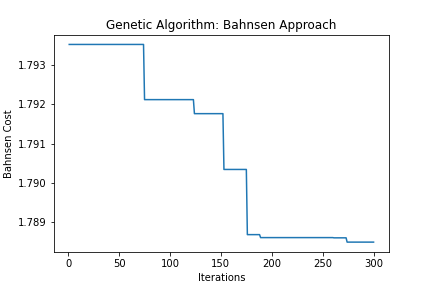
\includegraphics[width=0.8\textwidth]{bahnsen_plot.png}
    \caption{Genetic Algorithm Optimization for Bahnsen Approach}
\end{figure}

\section{Conclusion}
Both the Bahnsen and Nikou cost-sensitive approaches were implemented and optimized via a Genetic Algorithm. The results indicate that the GA effectively minimizes the cost-sensitive loss. Future work may refine these methods further for improved performance on larger datasets.

\end{document}